% WebKit / WKWebView data-collection architecture.
%
% Standalone:      pdflatex figures/webkit_architecture.tex
% Inside a paper:  \usepackage{standalone} in the preamble, then
%                  \begin{figure}% WebKit / WKWebView data-collection architecture.
%
% Standalone:      pdflatex figures/webkit_architecture.tex
% Inside a paper:  \usepackage{standalone} in the preamble, then
%                  \begin{figure}% WebKit / WKWebView data-collection architecture.
%
% Standalone:      pdflatex figures/webkit_architecture.tex
% Inside a paper:  \usepackage{standalone} in the preamble, then
%                  \begin{figure}% WebKit / WKWebView data-collection architecture.
%
% Standalone:      pdflatex figures/webkit_architecture.tex
% Inside a paper:  \usepackage{standalone} in the preamble, then
%                  \begin{figure}\input{figures/webkit_architecture}\end{figure}
\documentclass[tikz,border=8pt]{standalone}
\usepackage{lmodern}
\usepackage[T1]{fontenc}
\usetikzlibrary{arrows.meta,positioning,fit,backgrounds,calc,shapes.geometric}

% ---- palette -------------------------------------------------------------
\definecolor{nativeFill}{HTML}{E8EDF7}
\definecolor{nativeLine}{HTML}{3D5A94}
\definecolor{webkitFill}{HTML}{EFE7F6}
\definecolor{webkitLine}{HTML}{6B4C9A}
\definecolor{webFill}{HTML}{E3F2EF}
\definecolor{webLine}{HTML}{2E7D6F}
\definecolor{cloudFill}{HTML}{FDF0E3}
\definecolor{cloudLine}{HTML}{B5701C}
\definecolor{laneLine}{HTML}{9AA3AF}
\definecolor{flowLine}{HTML}{4B5563}

\begin{document}
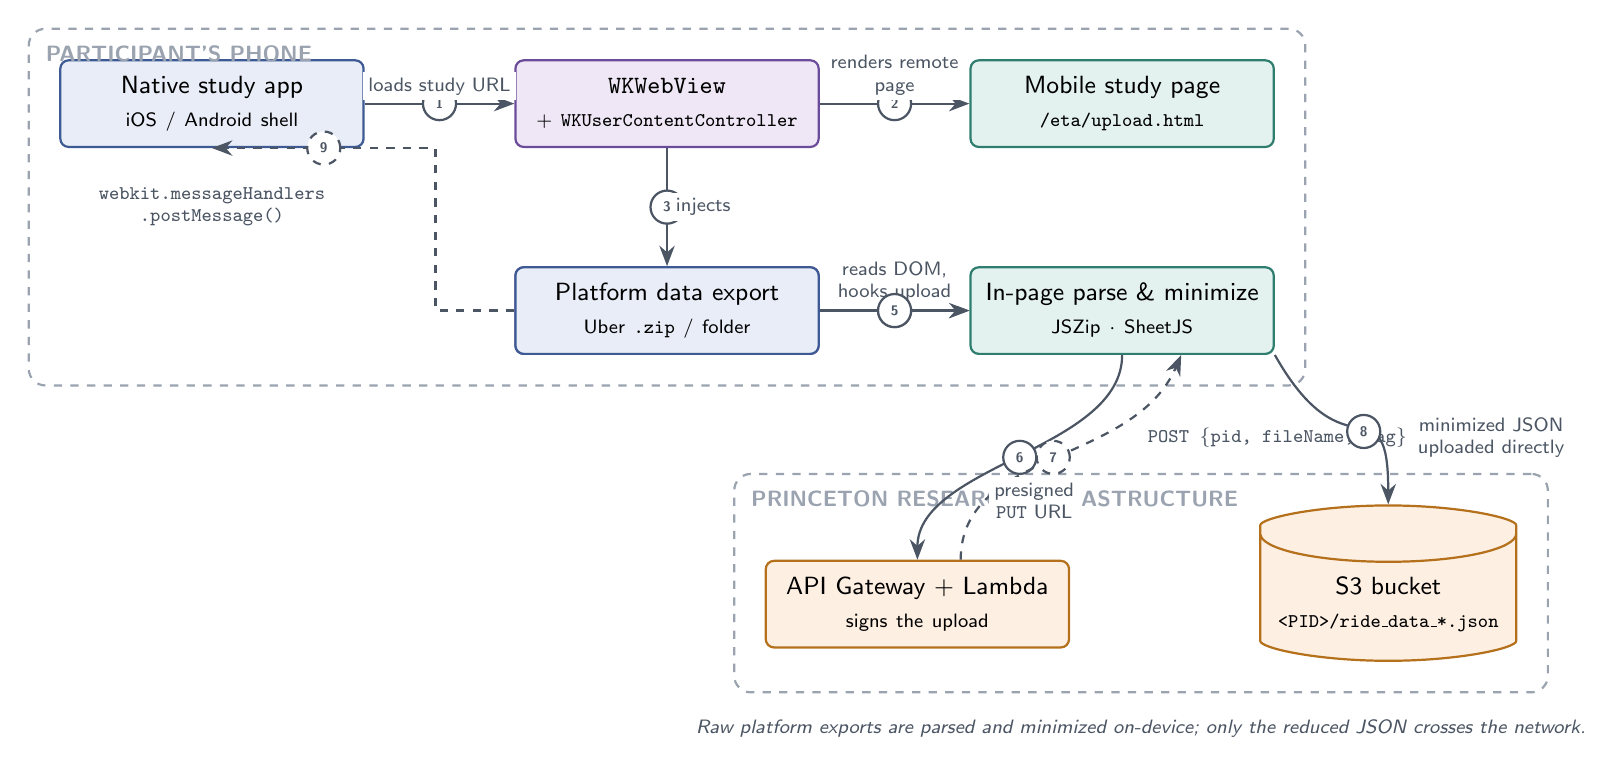
\begin{tikzpicture}[
  font=\sffamily\small,
  box/.style={
    draw, thick, rounded corners=3pt, align=center,
    minimum height=1.1cm, text width=3.5cm, inner sep=5pt},
  native/.style={box, fill=nativeFill, draw=nativeLine},
  webkit/.style={box, fill=webkitFill, draw=webkitLine},
  web/.style={box, fill=webFill, draw=webLine},
  cloud/.style={box, fill=cloudFill, draw=cloudLine},
  store/.style={cloud, cylinder, shape border rotate=90, aspect=0.22,
    text width=2.9cm, minimum height=1.3cm},
  flow/.style={-{Stealth[length=2.6mm]}, thick, draw=flowLine},
  back/.style={flow, dashed},
  lbl/.style={font=\sffamily\scriptsize, inner sep=2pt, fill=white,
    text=flowLine, align=center},
  stepnum/.style={circle, draw=flowLine, fill=white, thick, inner sep=0pt,
    minimum size=4.2mm, font=\sffamily\bfseries\tiny, text=flowLine},
  lane/.style={draw=laneLine, dashed, thick, rounded corners=6pt,
    inner sep=11pt},
  lanetag/.style={font=\sffamily\bfseries\footnotesize, text=laneLine},
]

% ===== device lane ========================================================
\node[native] (app) at (0,0)
  {Native study app\\[1pt]\scriptsize iOS / Android shell};

\node[webkit, right=1.9cm of app] (wk)
  {\texttt{WKWebView}\\[1pt]\scriptsize + \texttt{WKUserContentController}};

\node[web, right=1.9cm of wk] (page)
  {Mobile study page\\[1pt]\scriptsize\texttt{/eta/upload.html}};

\node[webkit, below=1.5cm of wk] (script)
  {Injected \texttt{WKUserScript}\\[1pt]\scriptsize\texttt{.atDocumentEnd}};

\node[web, below=1.5cm of page] (parse)
  {In-page parse \& minimize\\[1pt]\scriptsize JSZip $\cdot$ SheetJS};

\node[native, left=1.9cm of parse, yshift=0cm] (export)
  {Platform data export\\[1pt]\scriptsize Uber \texttt{.zip} / folder};

% ===== backend lane =======================================================
\node[cloud, below=2.6cm of parse, xshift=-2.6cm] (lambda)
  {API Gateway $+$ Lambda\\[1pt]\scriptsize signs the upload};

\node[store, right=2.4cm of lambda] (s3)
  {S3 bucket\\[1pt]\scriptsize\texttt{<PID>/ride\_data\_*.json}};

% ===== lane backgrounds ===================================================
\begin{scope}[on background layer]
  \node[lane, fit=(app)(page)(export)(parse)] (devlane) {};
  \node[lane, fit=(lambda)(s3)] (cloudlane) {};
\end{scope}
\node[lanetag, anchor=north west] at ($(devlane.north west)+(3pt,-3pt)$)
  {PARTICIPANT'S PHONE};
\node[lanetag, anchor=north west] at ($(cloudlane.north west)+(3pt,-3pt)$)
  {PRINCETON RESEARCH INFRASTRUCTURE};

% ===== flows ==============================================================
% 1. app -> webview
\draw[flow] (app) -- node[stepnum, pos=0.5] {1} (wk);
\node[lbl, above=1pt of $(app.east)!0.5!(wk.west)$] {loads study URL};

% 2. webview -> page
\draw[flow] (wk) -- node[stepnum, pos=0.5] {2} (page);
\node[lbl, above=1pt of $(wk.east)!0.5!(page.west)$] {renders remote\\page};

% 3. injection
\draw[flow] (wk) -- node[stepnum, pos=0.5] {3} (script);
\node[lbl, right=1pt of $(wk.south)!0.5!(script.north)$] {injects};

% 4. injected script drives the page
\draw[flow] (script) -- node[stepnum, pos=0.5] {4} (parse);
\node[lbl, above=1pt of $(script.east)!0.5!(parse.west)$] {reads DOM,\\hooks upload};

% 5. participant supplies the export
\draw[flow] (export) -- node[stepnum, pos=0.5] {5} (parse);

% 6. request presigned URL
\draw[flow] (parse.south) .. controls +(0,-1.2) and +(0,1.2) ..
  node[stepnum, pos=0.5] {6} (lambda.north);
\node[lbl, anchor=west] at ($(parse.south)+(0.25,-1.05)$)
  {\texttt{POST \{pid, fileName, tag\}}};

% 7. presigned URL returned
\draw[back] ($(lambda.north)+(0.55,0)$) .. controls +(0,1.4) and +(-0.6,-1.4) ..
  node[stepnum, pos=0.5] {7} ($(parse.south)+(0.75,0)$);
\node[lbl, anchor=west] at ($(lambda.north)+(0.9,0.75)$)
  {presigned\\\texttt{PUT} URL};

% 8. direct upload to S3
\draw[flow] (parse.south east) .. controls +(0.9,-1.6) and +(0,1.6) ..
  node[stepnum, pos=0.55] {8} (s3.north);
\node[lbl, anchor=west] at ($(s3.north)+(0.3,0.85)$)
  {minimized JSON\\uploaded directly};

% 9. completion message back to native
\draw[back] (script.west) -- ++(-1.0,0) |-
  node[stepnum, pos=0.75] {9} (app.south);
\node[lbl, anchor=north] at ($(app.south)+(0,-0.42)$)
  {\texttt{webkit.messageHandlers}\\\texttt{.postMessage()}};

% ===== note ===============================================================
\node[font=\sffamily\scriptsize\itshape, text=flowLine, align=center,
      below=6pt of cloudlane]
  {Raw platform exports are parsed and minimized on-device; only the reduced
   JSON crosses the network.};

\end{tikzpicture}
\end{document}
\end{figure}
\documentclass[tikz,border=8pt]{standalone}
\usepackage{lmodern}
\usepackage[T1]{fontenc}
\usetikzlibrary{arrows.meta,positioning,fit,backgrounds,calc,shapes.geometric}

% ---- palette -------------------------------------------------------------
\definecolor{nativeFill}{HTML}{E8EDF7}
\definecolor{nativeLine}{HTML}{3D5A94}
\definecolor{webkitFill}{HTML}{EFE7F6}
\definecolor{webkitLine}{HTML}{6B4C9A}
\definecolor{webFill}{HTML}{E3F2EF}
\definecolor{webLine}{HTML}{2E7D6F}
\definecolor{cloudFill}{HTML}{FDF0E3}
\definecolor{cloudLine}{HTML}{B5701C}
\definecolor{laneLine}{HTML}{9AA3AF}
\definecolor{flowLine}{HTML}{4B5563}

\begin{document}
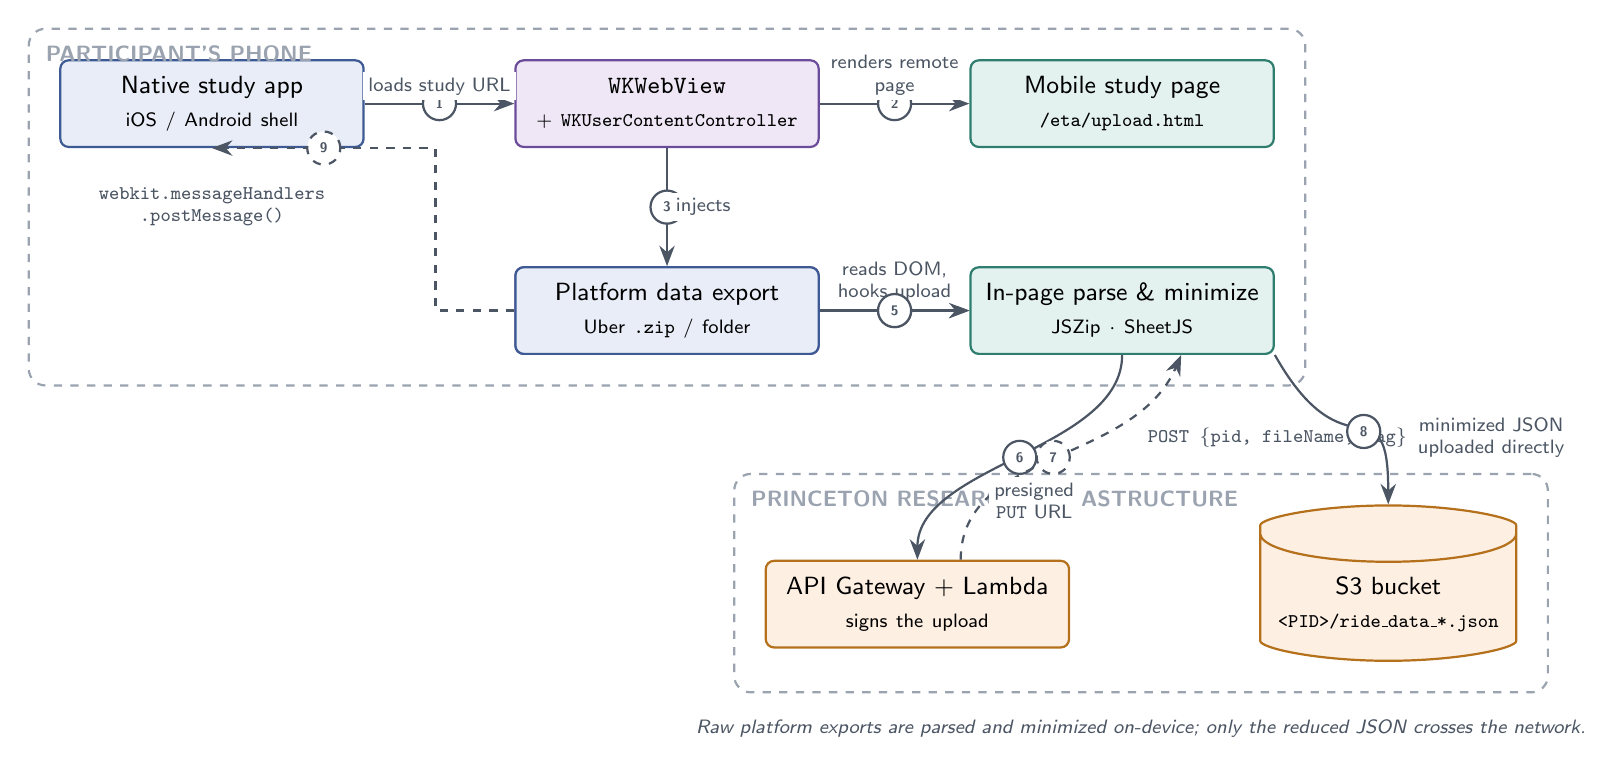
\begin{tikzpicture}[
  font=\sffamily\small,
  box/.style={
    draw, thick, rounded corners=3pt, align=center,
    minimum height=1.1cm, text width=3.5cm, inner sep=5pt},
  native/.style={box, fill=nativeFill, draw=nativeLine},
  webkit/.style={box, fill=webkitFill, draw=webkitLine},
  web/.style={box, fill=webFill, draw=webLine},
  cloud/.style={box, fill=cloudFill, draw=cloudLine},
  store/.style={cloud, cylinder, shape border rotate=90, aspect=0.22,
    text width=2.9cm, minimum height=1.3cm},
  flow/.style={-{Stealth[length=2.6mm]}, thick, draw=flowLine},
  back/.style={flow, dashed},
  lbl/.style={font=\sffamily\scriptsize, inner sep=2pt, fill=white,
    text=flowLine, align=center},
  stepnum/.style={circle, draw=flowLine, fill=white, thick, inner sep=0pt,
    minimum size=4.2mm, font=\sffamily\bfseries\tiny, text=flowLine},
  lane/.style={draw=laneLine, dashed, thick, rounded corners=6pt,
    inner sep=11pt},
  lanetag/.style={font=\sffamily\bfseries\footnotesize, text=laneLine},
]

% ===== device lane ========================================================
\node[native] (app) at (0,0)
  {Native study app\\[1pt]\scriptsize iOS / Android shell};

\node[webkit, right=1.9cm of app] (wk)
  {\texttt{WKWebView}\\[1pt]\scriptsize + \texttt{WKUserContentController}};

\node[web, right=1.9cm of wk] (page)
  {Mobile study page\\[1pt]\scriptsize\texttt{/eta/upload.html}};

\node[webkit, below=1.5cm of wk] (script)
  {Injected \texttt{WKUserScript}\\[1pt]\scriptsize\texttt{.atDocumentEnd}};

\node[web, below=1.5cm of page] (parse)
  {In-page parse \& minimize\\[1pt]\scriptsize JSZip $\cdot$ SheetJS};

\node[native, left=1.9cm of parse, yshift=0cm] (export)
  {Platform data export\\[1pt]\scriptsize Uber \texttt{.zip} / folder};

% ===== backend lane =======================================================
\node[cloud, below=2.6cm of parse, xshift=-2.6cm] (lambda)
  {API Gateway $+$ Lambda\\[1pt]\scriptsize signs the upload};

\node[store, right=2.4cm of lambda] (s3)
  {S3 bucket\\[1pt]\scriptsize\texttt{<PID>/ride\_data\_*.json}};

% ===== lane backgrounds ===================================================
\begin{scope}[on background layer]
  \node[lane, fit=(app)(page)(export)(parse)] (devlane) {};
  \node[lane, fit=(lambda)(s3)] (cloudlane) {};
\end{scope}
\node[lanetag, anchor=north west] at ($(devlane.north west)+(3pt,-3pt)$)
  {PARTICIPANT'S PHONE};
\node[lanetag, anchor=north west] at ($(cloudlane.north west)+(3pt,-3pt)$)
  {PRINCETON RESEARCH INFRASTRUCTURE};

% ===== flows ==============================================================
% 1. app -> webview
\draw[flow] (app) -- node[stepnum, pos=0.5] {1} (wk);
\node[lbl, above=1pt of $(app.east)!0.5!(wk.west)$] {loads study URL};

% 2. webview -> page
\draw[flow] (wk) -- node[stepnum, pos=0.5] {2} (page);
\node[lbl, above=1pt of $(wk.east)!0.5!(page.west)$] {renders remote\\page};

% 3. injection
\draw[flow] (wk) -- node[stepnum, pos=0.5] {3} (script);
\node[lbl, right=1pt of $(wk.south)!0.5!(script.north)$] {injects};

% 4. injected script drives the page
\draw[flow] (script) -- node[stepnum, pos=0.5] {4} (parse);
\node[lbl, above=1pt of $(script.east)!0.5!(parse.west)$] {reads DOM,\\hooks upload};

% 5. participant supplies the export
\draw[flow] (export) -- node[stepnum, pos=0.5] {5} (parse);

% 6. request presigned URL
\draw[flow] (parse.south) .. controls +(0,-1.2) and +(0,1.2) ..
  node[stepnum, pos=0.5] {6} (lambda.north);
\node[lbl, anchor=west] at ($(parse.south)+(0.25,-1.05)$)
  {\texttt{POST \{pid, fileName, tag\}}};

% 7. presigned URL returned
\draw[back] ($(lambda.north)+(0.55,0)$) .. controls +(0,1.4) and +(-0.6,-1.4) ..
  node[stepnum, pos=0.5] {7} ($(parse.south)+(0.75,0)$);
\node[lbl, anchor=west] at ($(lambda.north)+(0.9,0.75)$)
  {presigned\\\texttt{PUT} URL};

% 8. direct upload to S3
\draw[flow] (parse.south east) .. controls +(0.9,-1.6) and +(0,1.6) ..
  node[stepnum, pos=0.55] {8} (s3.north);
\node[lbl, anchor=west] at ($(s3.north)+(0.3,0.85)$)
  {minimized JSON\\uploaded directly};

% 9. completion message back to native
\draw[back] (script.west) -- ++(-1.0,0) |-
  node[stepnum, pos=0.75] {9} (app.south);
\node[lbl, anchor=north] at ($(app.south)+(0,-0.42)$)
  {\texttt{webkit.messageHandlers}\\\texttt{.postMessage()}};

% ===== note ===============================================================
\node[font=\sffamily\scriptsize\itshape, text=flowLine, align=center,
      below=6pt of cloudlane]
  {Raw platform exports are parsed and minimized on-device; only the reduced
   JSON crosses the network.};

\end{tikzpicture}
\end{document}
\end{figure}
\documentclass[tikz,border=8pt]{standalone}
\usepackage{lmodern}
\usepackage[T1]{fontenc}
\usetikzlibrary{arrows.meta,positioning,fit,backgrounds,calc,shapes.geometric}

% ---- palette -------------------------------------------------------------
\definecolor{nativeFill}{HTML}{E8EDF7}
\definecolor{nativeLine}{HTML}{3D5A94}
\definecolor{webkitFill}{HTML}{EFE7F6}
\definecolor{webkitLine}{HTML}{6B4C9A}
\definecolor{webFill}{HTML}{E3F2EF}
\definecolor{webLine}{HTML}{2E7D6F}
\definecolor{cloudFill}{HTML}{FDF0E3}
\definecolor{cloudLine}{HTML}{B5701C}
\definecolor{laneLine}{HTML}{9AA3AF}
\definecolor{flowLine}{HTML}{4B5563}

\begin{document}
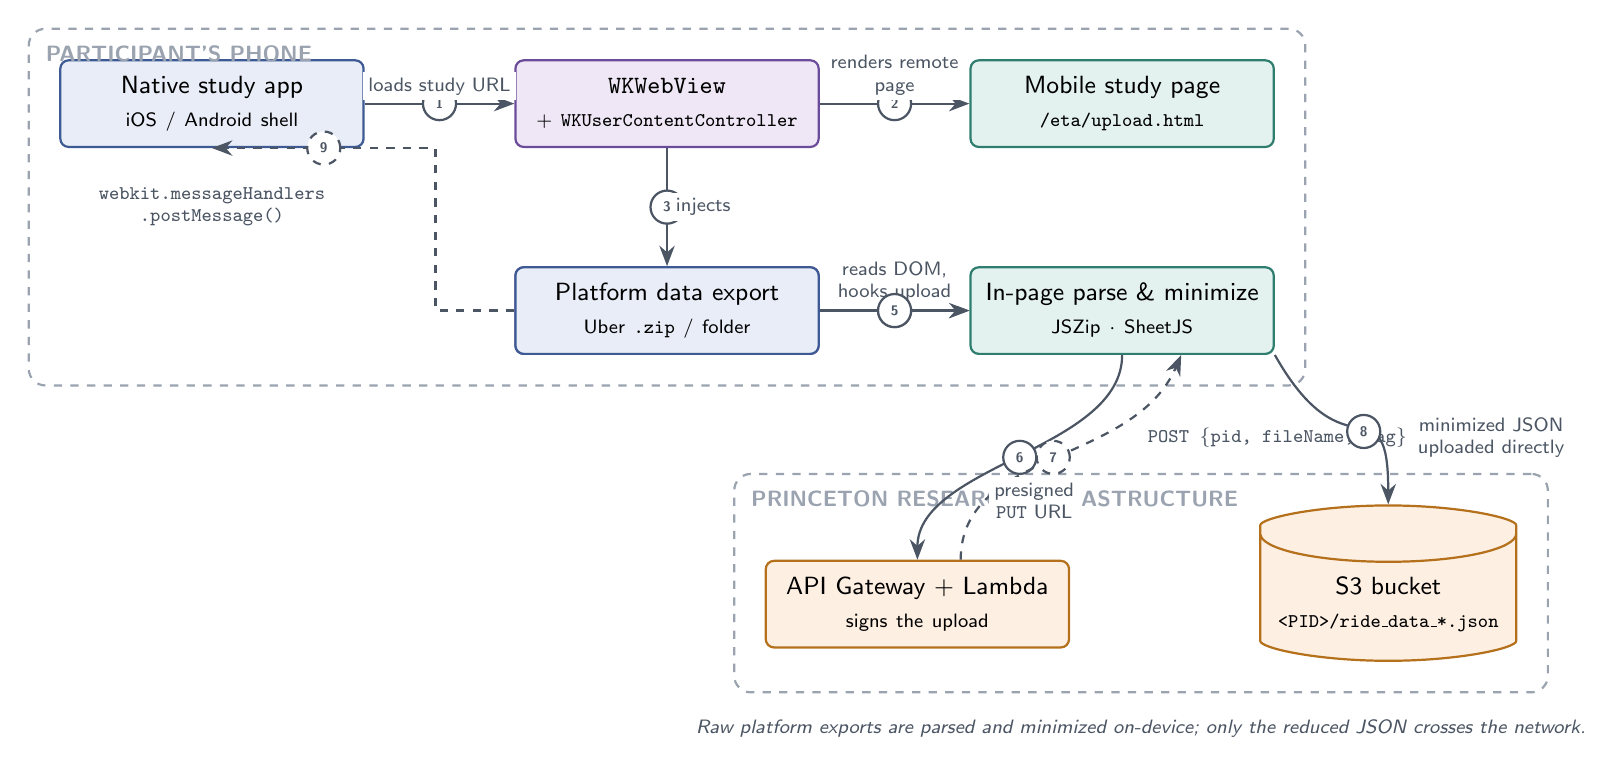
\begin{tikzpicture}[
  font=\sffamily\small,
  box/.style={
    draw, thick, rounded corners=3pt, align=center,
    minimum height=1.1cm, text width=3.5cm, inner sep=5pt},
  native/.style={box, fill=nativeFill, draw=nativeLine},
  webkit/.style={box, fill=webkitFill, draw=webkitLine},
  web/.style={box, fill=webFill, draw=webLine},
  cloud/.style={box, fill=cloudFill, draw=cloudLine},
  store/.style={cloud, cylinder, shape border rotate=90, aspect=0.22,
    text width=2.9cm, minimum height=1.3cm},
  flow/.style={-{Stealth[length=2.6mm]}, thick, draw=flowLine},
  back/.style={flow, dashed},
  lbl/.style={font=\sffamily\scriptsize, inner sep=2pt, fill=white,
    text=flowLine, align=center},
  stepnum/.style={circle, draw=flowLine, fill=white, thick, inner sep=0pt,
    minimum size=4.2mm, font=\sffamily\bfseries\tiny, text=flowLine},
  lane/.style={draw=laneLine, dashed, thick, rounded corners=6pt,
    inner sep=11pt},
  lanetag/.style={font=\sffamily\bfseries\footnotesize, text=laneLine},
]

% ===== device lane ========================================================
\node[native] (app) at (0,0)
  {Native study app\\[1pt]\scriptsize iOS / Android shell};

\node[webkit, right=1.9cm of app] (wk)
  {\texttt{WKWebView}\\[1pt]\scriptsize + \texttt{WKUserContentController}};

\node[web, right=1.9cm of wk] (page)
  {Mobile study page\\[1pt]\scriptsize\texttt{/eta/upload.html}};

\node[webkit, below=1.5cm of wk] (script)
  {Injected \texttt{WKUserScript}\\[1pt]\scriptsize\texttt{.atDocumentEnd}};

\node[web, below=1.5cm of page] (parse)
  {In-page parse \& minimize\\[1pt]\scriptsize JSZip $\cdot$ SheetJS};

\node[native, left=1.9cm of parse, yshift=0cm] (export)
  {Platform data export\\[1pt]\scriptsize Uber \texttt{.zip} / folder};

% ===== backend lane =======================================================
\node[cloud, below=2.6cm of parse, xshift=-2.6cm] (lambda)
  {API Gateway $+$ Lambda\\[1pt]\scriptsize signs the upload};

\node[store, right=2.4cm of lambda] (s3)
  {S3 bucket\\[1pt]\scriptsize\texttt{<PID>/ride\_data\_*.json}};

% ===== lane backgrounds ===================================================
\begin{scope}[on background layer]
  \node[lane, fit=(app)(page)(export)(parse)] (devlane) {};
  \node[lane, fit=(lambda)(s3)] (cloudlane) {};
\end{scope}
\node[lanetag, anchor=north west] at ($(devlane.north west)+(3pt,-3pt)$)
  {PARTICIPANT'S PHONE};
\node[lanetag, anchor=north west] at ($(cloudlane.north west)+(3pt,-3pt)$)
  {PRINCETON RESEARCH INFRASTRUCTURE};

% ===== flows ==============================================================
% 1. app -> webview
\draw[flow] (app) -- node[stepnum, pos=0.5] {1} (wk);
\node[lbl, above=1pt of $(app.east)!0.5!(wk.west)$] {loads study URL};

% 2. webview -> page
\draw[flow] (wk) -- node[stepnum, pos=0.5] {2} (page);
\node[lbl, above=1pt of $(wk.east)!0.5!(page.west)$] {renders remote\\page};

% 3. injection
\draw[flow] (wk) -- node[stepnum, pos=0.5] {3} (script);
\node[lbl, right=1pt of $(wk.south)!0.5!(script.north)$] {injects};

% 4. injected script drives the page
\draw[flow] (script) -- node[stepnum, pos=0.5] {4} (parse);
\node[lbl, above=1pt of $(script.east)!0.5!(parse.west)$] {reads DOM,\\hooks upload};

% 5. participant supplies the export
\draw[flow] (export) -- node[stepnum, pos=0.5] {5} (parse);

% 6. request presigned URL
\draw[flow] (parse.south) .. controls +(0,-1.2) and +(0,1.2) ..
  node[stepnum, pos=0.5] {6} (lambda.north);
\node[lbl, anchor=west] at ($(parse.south)+(0.25,-1.05)$)
  {\texttt{POST \{pid, fileName, tag\}}};

% 7. presigned URL returned
\draw[back] ($(lambda.north)+(0.55,0)$) .. controls +(0,1.4) and +(-0.6,-1.4) ..
  node[stepnum, pos=0.5] {7} ($(parse.south)+(0.75,0)$);
\node[lbl, anchor=west] at ($(lambda.north)+(0.9,0.75)$)
  {presigned\\\texttt{PUT} URL};

% 8. direct upload to S3
\draw[flow] (parse.south east) .. controls +(0.9,-1.6) and +(0,1.6) ..
  node[stepnum, pos=0.55] {8} (s3.north);
\node[lbl, anchor=west] at ($(s3.north)+(0.3,0.85)$)
  {minimized JSON\\uploaded directly};

% 9. completion message back to native
\draw[back] (script.west) -- ++(-1.0,0) |-
  node[stepnum, pos=0.75] {9} (app.south);
\node[lbl, anchor=north] at ($(app.south)+(0,-0.42)$)
  {\texttt{webkit.messageHandlers}\\\texttt{.postMessage()}};

% ===== note ===============================================================
\node[font=\sffamily\scriptsize\itshape, text=flowLine, align=center,
      below=6pt of cloudlane]
  {Raw platform exports are parsed and minimized on-device; only the reduced
   JSON crosses the network.};

\end{tikzpicture}
\end{document}
\end{figure}
\documentclass[tikz,border=8pt]{standalone}
\usepackage{lmodern}
\usepackage[T1]{fontenc}
\usetikzlibrary{arrows.meta,positioning,fit,backgrounds,calc,shapes.geometric}

% ---- palette -------------------------------------------------------------
\definecolor{nativeFill}{HTML}{E8EDF7}
\definecolor{nativeLine}{HTML}{3D5A94}
\definecolor{webkitFill}{HTML}{EFE7F6}
\definecolor{webkitLine}{HTML}{6B4C9A}
\definecolor{webFill}{HTML}{E3F2EF}
\definecolor{webLine}{HTML}{2E7D6F}
\definecolor{cloudFill}{HTML}{FDF0E3}
\definecolor{cloudLine}{HTML}{B5701C}
\definecolor{laneLine}{HTML}{9AA3AF}
\definecolor{flowLine}{HTML}{4B5563}

\begin{document}
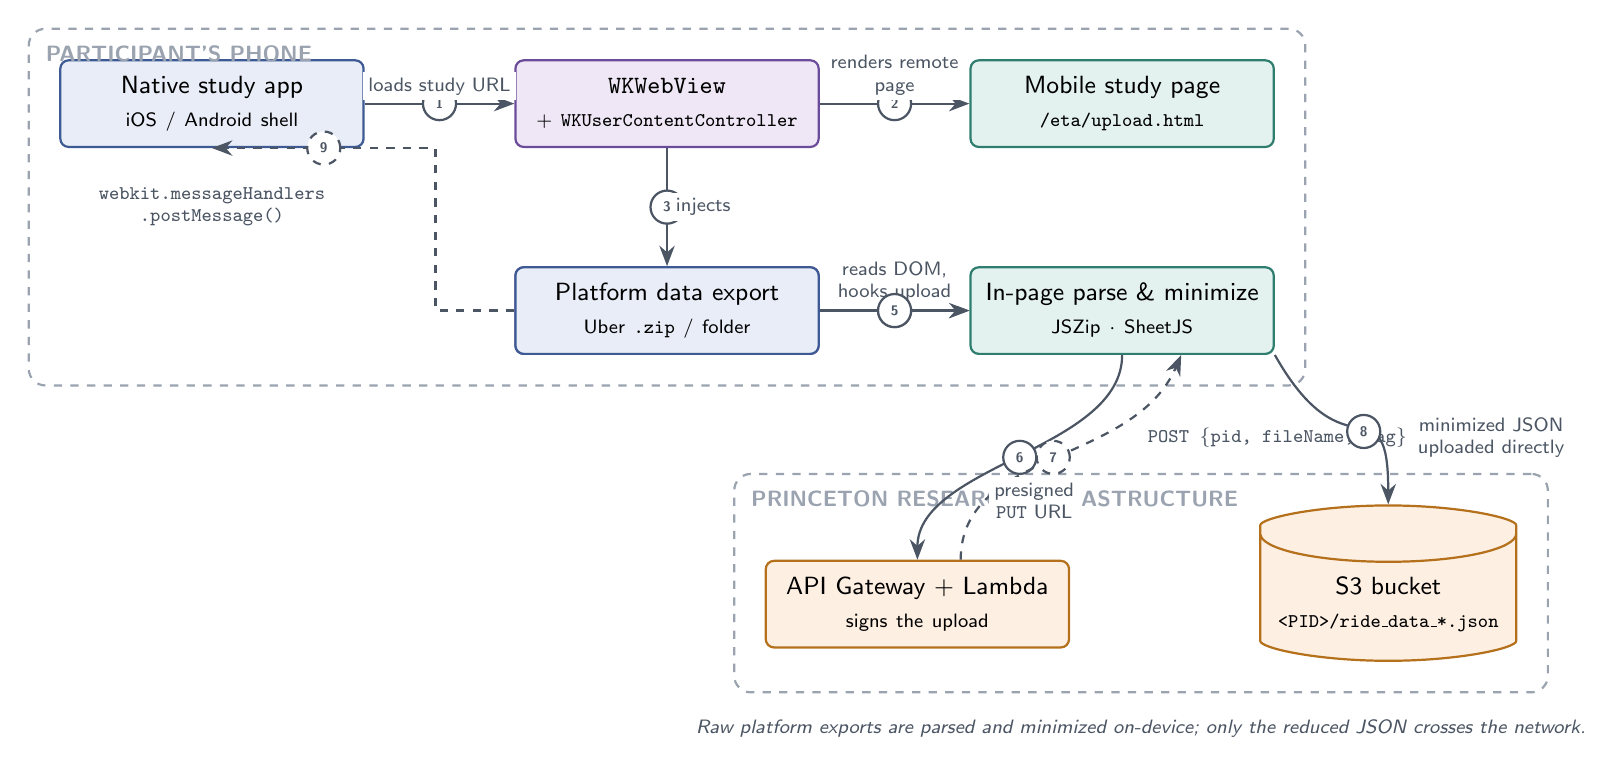
\begin{tikzpicture}[
  font=\sffamily\small,
  box/.style={
    draw, thick, rounded corners=3pt, align=center,
    minimum height=1.1cm, text width=3.5cm, inner sep=5pt},
  native/.style={box, fill=nativeFill, draw=nativeLine},
  webkit/.style={box, fill=webkitFill, draw=webkitLine},
  web/.style={box, fill=webFill, draw=webLine},
  cloud/.style={box, fill=cloudFill, draw=cloudLine},
  store/.style={cloud, cylinder, shape border rotate=90, aspect=0.22,
    text width=2.9cm, minimum height=1.3cm},
  flow/.style={-{Stealth[length=2.6mm]}, thick, draw=flowLine},
  back/.style={flow, dashed},
  lbl/.style={font=\sffamily\scriptsize, inner sep=2pt, fill=white,
    text=flowLine, align=center},
  stepnum/.style={circle, draw=flowLine, fill=white, thick, inner sep=0pt,
    minimum size=4.2mm, font=\sffamily\bfseries\tiny, text=flowLine},
  lane/.style={draw=laneLine, dashed, thick, rounded corners=6pt,
    inner sep=11pt},
  lanetag/.style={font=\sffamily\bfseries\footnotesize, text=laneLine},
]

% ===== device lane ========================================================
\node[native] (app) at (0,0)
  {Native study app\\[1pt]\scriptsize iOS / Android shell};

\node[webkit, right=1.9cm of app] (wk)
  {\texttt{WKWebView}\\[1pt]\scriptsize + \texttt{WKUserContentController}};

\node[web, right=1.9cm of wk] (page)
  {Mobile study page\\[1pt]\scriptsize\texttt{/eta/upload.html}};

\node[webkit, below=1.5cm of wk] (script)
  {Injected \texttt{WKUserScript}\\[1pt]\scriptsize\texttt{.atDocumentEnd}};

\node[web, below=1.5cm of page] (parse)
  {In-page parse \& minimize\\[1pt]\scriptsize JSZip $\cdot$ SheetJS};

\node[native, left=1.9cm of parse, yshift=0cm] (export)
  {Platform data export\\[1pt]\scriptsize Uber \texttt{.zip} / folder};

% ===== backend lane =======================================================
\node[cloud, below=2.6cm of parse, xshift=-2.6cm] (lambda)
  {API Gateway $+$ Lambda\\[1pt]\scriptsize signs the upload};

\node[store, right=2.4cm of lambda] (s3)
  {S3 bucket\\[1pt]\scriptsize\texttt{<PID>/ride\_data\_*.json}};

% ===== lane backgrounds ===================================================
\begin{scope}[on background layer]
  \node[lane, fit=(app)(page)(export)(parse)] (devlane) {};
  \node[lane, fit=(lambda)(s3)] (cloudlane) {};
\end{scope}
\node[lanetag, anchor=north west] at ($(devlane.north west)+(3pt,-3pt)$)
  {PARTICIPANT'S PHONE};
\node[lanetag, anchor=north west] at ($(cloudlane.north west)+(3pt,-3pt)$)
  {PRINCETON RESEARCH INFRASTRUCTURE};

% ===== flows ==============================================================
% 1. app -> webview
\draw[flow] (app) -- node[stepnum, pos=0.5] {1} (wk);
\node[lbl, above=1pt of $(app.east)!0.5!(wk.west)$] {loads study URL};

% 2. webview -> page
\draw[flow] (wk) -- node[stepnum, pos=0.5] {2} (page);
\node[lbl, above=1pt of $(wk.east)!0.5!(page.west)$] {renders remote\\page};

% 3. injection
\draw[flow] (wk) -- node[stepnum, pos=0.5] {3} (script);
\node[lbl, right=1pt of $(wk.south)!0.5!(script.north)$] {injects};

% 4. injected script drives the page
\draw[flow] (script) -- node[stepnum, pos=0.5] {4} (parse);
\node[lbl, above=1pt of $(script.east)!0.5!(parse.west)$] {reads DOM,\\hooks upload};

% 5. participant supplies the export
\draw[flow] (export) -- node[stepnum, pos=0.5] {5} (parse);

% 6. request presigned URL
\draw[flow] (parse.south) .. controls +(0,-1.2) and +(0,1.2) ..
  node[stepnum, pos=0.5] {6} (lambda.north);
\node[lbl, anchor=west] at ($(parse.south)+(0.25,-1.05)$)
  {\texttt{POST \{pid, fileName, tag\}}};

% 7. presigned URL returned
\draw[back] ($(lambda.north)+(0.55,0)$) .. controls +(0,1.4) and +(-0.6,-1.4) ..
  node[stepnum, pos=0.5] {7} ($(parse.south)+(0.75,0)$);
\node[lbl, anchor=west] at ($(lambda.north)+(0.9,0.75)$)
  {presigned\\\texttt{PUT} URL};

% 8. direct upload to S3
\draw[flow] (parse.south east) .. controls +(0.9,-1.6) and +(0,1.6) ..
  node[stepnum, pos=0.55] {8} (s3.north);
\node[lbl, anchor=west] at ($(s3.north)+(0.3,0.85)$)
  {minimized JSON\\uploaded directly};

% 9. completion message back to native
\draw[back] (script.west) -- ++(-1.0,0) |-
  node[stepnum, pos=0.75] {9} (app.south);
\node[lbl, anchor=north] at ($(app.south)+(0,-0.42)$)
  {\texttt{webkit.messageHandlers}\\\texttt{.postMessage()}};

% ===== note ===============================================================
\node[font=\sffamily\scriptsize\itshape, text=flowLine, align=center,
      below=6pt of cloudlane]
  {Raw platform exports are parsed and minimized on-device; only the reduced
   JSON crosses the network.};

\end{tikzpicture}
\end{document}
